\section{Fault tolerance design}
This section describes the design of the archive service in case of different kinds of failures. The system being part of a large distributed system,
faces different difficult situation which must be handled for a better. Table \ref{table:probServices} lists the possible errors which 
could occur with a brief description.i.e. network issues, failure of a 
dependent service, sudden termination of the archive service 
\begin{longtable}{|p{4cm}|p{10cm}|}
    \hline
        \textbf{Errors}  & \textbf{Description}\\
    \hline
        Network glitches & The MARS framework is built upon a complex Distributed System architecture and the communication between the services
        happen via a network (e.g HTTP, RPC). It is a possibility that the connection cannot be established for a small period of time due to some network problems.
        This would lead the archive service to fail even though all the services are functioning.\\
    \hline
        Failure of a dependent service & There is a possibility that a service that the archive service is dependent upon goes down temporarily due to an unexpected
        failure or due to maintenance purpose. The failure of the dependent service to answer would also generate an error in the Archive service.\\
    \hline
        Sudden failure of the Archive service & As for other services the archive service is also prone for getting an unexpected restart. This restart would cause
        the running job to stop and the progress being lost.\\    
    \hline
    \caption{Possible errors which could occur in the Archive service}
    \label{table:probServices} 
\end{longtable}

Figure \ref{fig:activityFailure} illustrates the activity diagram which describes how the Archive service will be designed so that a recovery from errors mentioned in
Table \ref{table:probServices} could be handled. The main strategy for the failure mitigation is to re run the process again from the beginning once an error occurs. 
The important that the necessary parameters which is required for the successful start of the process i.e. input parameters, retry counters, start time are persisted
in a database. Storing these data in the database would mean that the in case of a system failure the service can fetch all the required parameters and restart the 
process automatically. The number of restarts can be configured by the programmer. This is designed in such a way so that the service avoids a deadlock situation of the
resource being restarted infinitely. Additionally, a cumulative wait time for the restart can also be added so that there is some gap between the process restart.

\begin{figure}[H]
    \centering 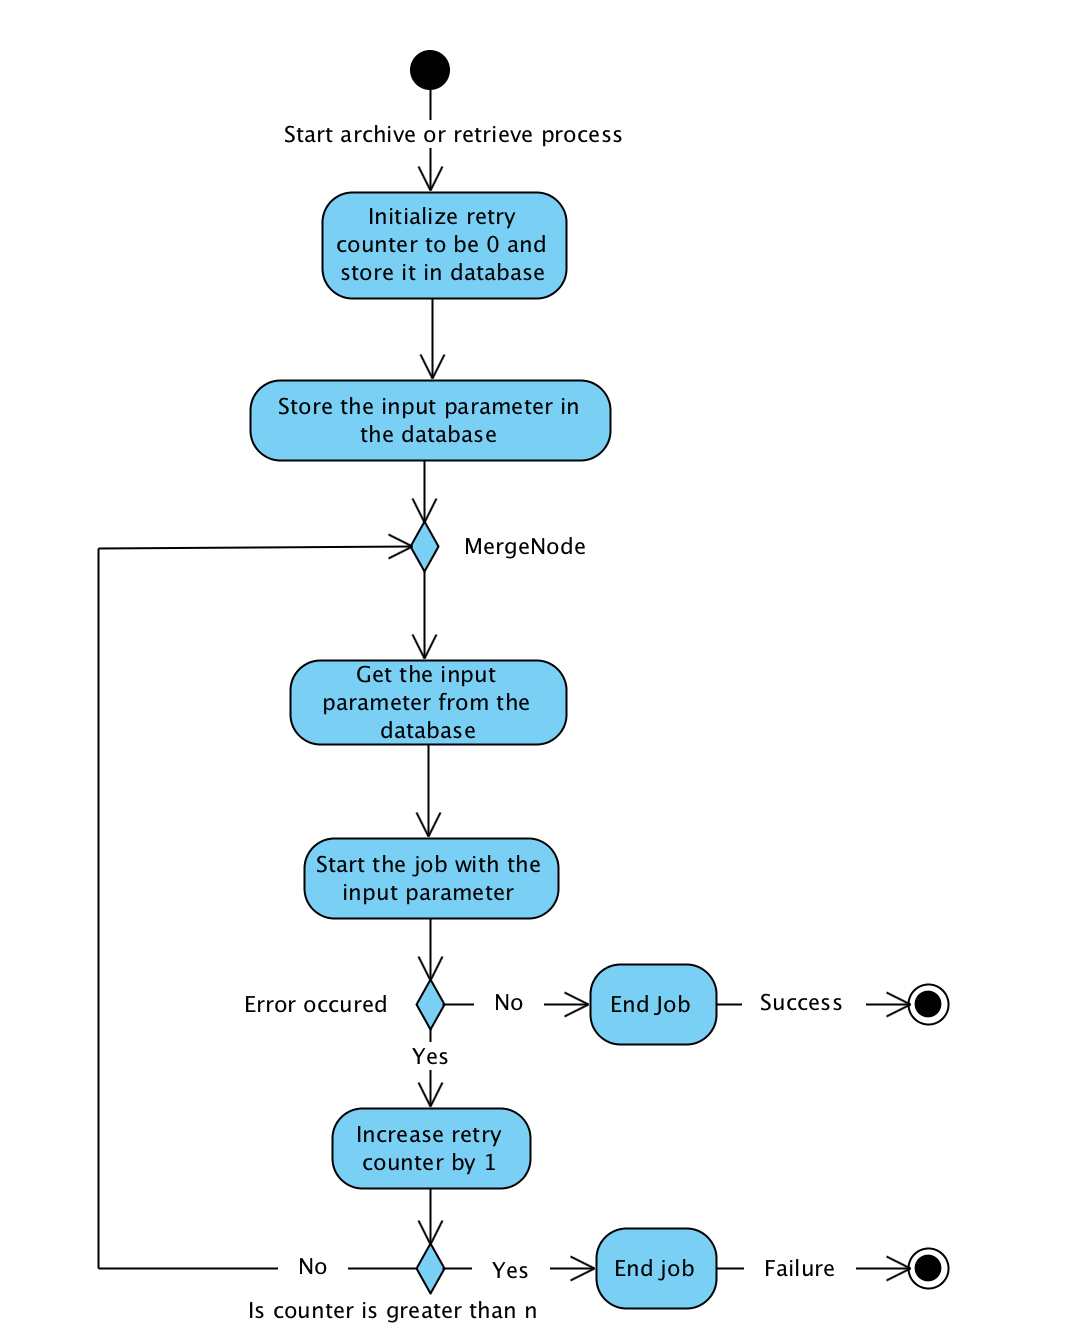
\includegraphics[scale=0.6]{grafiken/activityFailure.png}
    \caption{Activity Diagram for failure mitigation for the Archive service \cite{Hangfire}}
    \label{fig:activityFailure}
\end{figure}
